\chapauthor{Самодумкин С.А.}
\chapter{Подсистема Экосистемы OSTIS, обеспечивающая поддержку жизненного цикла интеллектуальных геоинформационных систем различного назначения}
\chapauthortoc{Самодумкин С.А.}
\label{chapter_gis}

\abstract{Аннотация к главе.}

\section{Требования, предъявляемые к интеллектуальным геоинформационным системам нового поколения}
\section{Систематизация задач, решаемых интеллектуальными геоинформационными системами}
\section{Основные компоненты формальных онтологий, используемых в геоинформационных системах}
\label{gis_components}

\begin{figure}[H]
	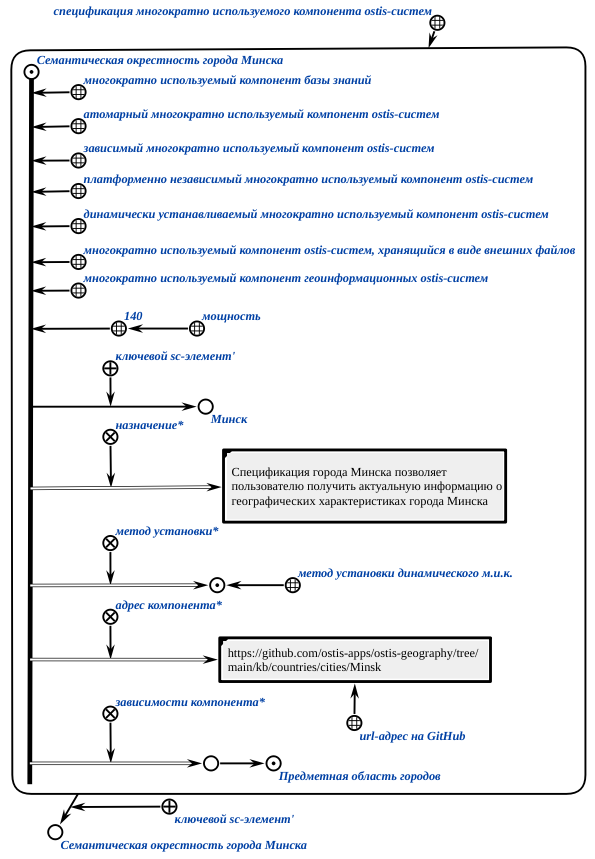
\includegraphics[scale=0.8]{author/part7/figures/gis_kb_component.png}
	@@ -22,11 +443,4 @@ \section{Основные компоненты формальных онтоло
	\label{fig:gis_ps_component}
\end{figure}

\subsection{Геосемантические элементы: местоположение, топология, близость, ориентация, динамика}
\subsection{Формализация пространственных отношений в геоинформационных системах}
\section{Стратифицированная модель информационного пространства объектов местности}
\section{Формальная денотационная семантика языка карт}
\section{Формальная онтология объектов местности}
\section{Средства автоматизации проектирования интеллектуальных геоинформационных систем}

